\documentclass[12pt,a4paper]{article}

\usepackage[pdftex, bookmarks=true,unicode=true, colorlinks=true, 
linkcolor=red, citecolor=green, filecolor=magenta, urlcolor=cyan, breaklinks 
]{hyperref}
%\usepackage{subfigure}
\usepackage{graphics}
\usepackage{graphicx}
\usepackage{caption}  % Formatierung von Bild-/Tabellentiteln
           
\usepackage[T1]{fontenc}           
\usepackage[utf8]{inputenc}
\usepackage[english,ngerman]{babel}
\usepackage{color}
\usepackage{amsmath,amssymb,amsfonts}				% AMS symbols
\usepackage{listings}
\usepackage{notoccite}
\usepackage{verbatim}
\usepackage{sverb}
\usepackage{ifthen}
\usepackage{fancyhdr}
\usepackage{float}
\usepackage{tocbibind}
\usepackage{titling}
\usepackage{acronym}
\usepackage[binary-units]{siunitx}
\usepackage{cleveref}
\usepackage{listings}
% \usepackage{breakurl}

\usepackage[numbered]{bookmark}

\sisetup{
  range-phrase = --,
  range-units = single
}

\acrodefplural{GPU}[GPUs]{Graphics Processing Units}

\lstset{
  basicstyle=\footnotesize
}

\lstdefinelanguage{OpenCL}{%
  language=C,
  morekeywords={kernel,__kernel,local,__local,global,__global,private,__private,
                get_local_id,get_global_id,get_group_id,constant,__constant}
}

\newcommand{\thesistitle}{\iflanguage{english}{Automatic optimization of linear 
algebra routines for heterogeneous systems}{Automatische Optimierung von 
Grundoperationen der linearen Algebra für heterogene Systeme}}

\newcommand{\correctlanguage} { \selectlanguage{english} }

\newcommand\thecategory {}
\newcommand*{\category}[1]{\renewcommand\thecategory{#1}}


%\renewcommand{\chaptermark}[1]{\markright{\chaptername {} \thechapter:  #1}{}}
\renewcommand{\sectionmark}[1]{\markright{\thesection\ #1}}

\setkeys{Gin}{keepaspectratio=true}
\widowpenalty=1000
\clubpenalty=1000
\setcounter{secnumdepth}{3}
\renewcommand{\textfraction}{0}
\renewcommand{\topfraction}{0.75}
\renewcommand{\bottomfraction}{0.75}
\renewcommand{\floatpagefraction}{0.8}
\restylefloat{float}
\pagestyle{fancy}
\lhead[\fancyplain{}{\bf\thepage}]{\fancyplain{}{\let\uppercase\relax\rightmark}}
\chead{}
\rhead[\fancyplain{}{\bf\thepage}]{\fancyplain{}{\thepage}}
\lfoot{}
\cfoot{}
\rfoot[]{}%
\addtolength{\headheight}{1cm}  % Headerhöhe vergrößern, sonst Fehlermeldung

\correctlanguage

%----------------------------------------------------------------------
%- Set document parameters
%---------------------------------------------------------------------

\hypersetup{%
    pdftitle={\thesistitle},    % title
    pdfauthor={Felix Patschkowski},     % author
    pdfsubject={Project Name},   % subject of the document
    pdfkeywords= {Keywords}, % list of keywords
}

\DeclareGraphicsExtensions{.pdf,.png,.jpg,.jpeg}

\graphicspath{{figures/}}

%----------------------------------------------------------------------
%- Set title page
%---------------------------------------------------------------------

\title{\thesistitle}
\author{Felix Patschkowski (43191)}
\date{\today}
\category{Project Thesis}

\hyphenation{In-ter-pre-ter Diag-nos-tik A-no-de}

%----------------------------------------------------------------------
%- Documentation
%---------------------------------------------------------------------

\begin{document}

\cleardoublepage
\begin{titlepage}

\begin{tabular}{lcr}

\includegraphics[width=7cm]{TUHH_print2} & \hspace{1cm} & 
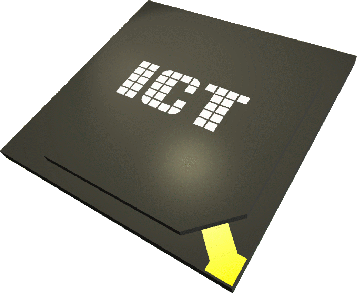
\includegraphics[width=3cm]{ICT_print}
\end{tabular}
\vfill%
\begin{center}%
\Large%
Technische Universität Hamburg-Harburg\\
Institut für Rechnertechnologie\par
Prof. Dr. F. Mayer-Lindenberg\par
\vspace{3cm}
\vfill%
{\huge \bf \thetitle \par % \@title
\vspace{1.2cm}
\vfill
\Large
\thecategory\\ % \thecategory
\vspace{0mm}
\theauthor \par % @author
\vspace{6mm}
\vfill
}
\Large
\thedate\par%\@date
\vspace{0.5cm}
\normalsize
%\theremark
\end{center}
\end{titlepage}

\cleardoublepage

\correctlanguage

%\chapter*{\iflanguage{english}{Project description}{Aufgabenstellung}}

\begin{center} \section*{\iflanguage{english}{Project description}{Aufgabenstellung}} \end{center}
\thispagestyle{empty}           % Seite nicht numerieren
{

%------------------------------
% Formatierung
%------------------------------
\setlength{\parindent}{0mm}     % Absatzanfänge nicht einrücken
\setlength{\topmargin}{1mm}
\setlength{\topskip}{1mm}
\setlength{\headheight}{1mm}
\setlength{\headsep}{1mm}


%------------------------------
% Briefkopf
%------------------------------
\begin{center}
		 Technische Universität Hamburg-Harburg\\
		 Institut für Rechnertechnologie\\
		 Prof. Dr. F. Mayer-Lindenberg\\[10mm]
		 \textbf{Aufgabenstellung der Studienarbeit/Diplomarbeit\\[2,5mm]
		 \large Automatische Optimierung von Grundoperationen der 
linearen Algebra auf heterogenen Rechensystemen}
\end{center}


%------------------------------
% Aufgabe
%------------------------------
\small {\iflanguage{english}{Project description}{Beschreibung der Aufgabe}} 



%------------------------------
% Daten und Unterschrift
%------------------------------

\begin{tabbing}
  Betreuer\quad\quad\quad\quad\=: Dipl. Ing. Cem Bassoy\\
  Referent\>: Professor F. Mayer-Lindenberg \\
  Ausgabedatum\>: 01. Mai 2014\\
  Bearbeitungszeit\>: 6 Monate
\end{tabbing}

%\vfill
%\begin{flushright}
%		 .........................................................\\
%		 Professor
%\end{flushright}
}
\newpage


%\chapter*{\iflanguage{english}{Declaration}{Erklärung}}
\section*{\iflanguage{english}{Declaration}{Erklärung}}  
\thispagestyle{empty}           % Seite nicht numerieren
{
\setlength{\parindent}{0mm}		 		 % Absatzanfänge nicht einrücken
\iflanguage{english}%
{This project is the result of my own work, except where explicit reference is made to the work of others, and has not been submitted
for another qualification to this or any other university.}%
{Hiermit erkläre ich, dass die vorliegende Arbeit von mir selbständig und nur 
unter Verwendung der aufgeführten Hilfsmittel erstellt wurde.}

\vspace{2cm}

Hamburg, \today
} % \parindent
\newpage


%\chapter*{\iflanguage{english}{Acknowledgements}{Danksagung}}
\section*{\iflanguage{english}{Acknowledgements}{Danksagung}}
\thispagestyle{empty}
{
\setlength{\parindent}{0mm}
} % \parindent
\newpage


\correctlanguage

\pagenumbering{roman} 

\correctlanguage

\tableofcontents
\cleardoublepage
\listoffigures
\cleardoublepage
\listoftables
\cleardoublepage


%----------------------------------------------------------------------
%- Include your own Chapters 
%----------------------------------------------------------------------
\pagenumbering{arabic}
\setcounter{page}{1}

%\chapter*{\iflanguage{english}{Abstract}{Zusammenfassung}}
\section*{\iflanguage{english}{Abstract}{Zusammenfassung}}
\newpage


\section{Einleitung}  \label{chap:einleitung}


\section{\iflanguage{english}{Previous Work}{Frühere Arbeiten}}
This section summarizes previous and related work from selected papers.

In 2008 Volkov and Demmel examined in \cite{Volkov2008} the characteristics of 
back than recent NVIDIA \acp{GPU}\footnote{GeForce 8, 9 and 200 series} using 
microbenchmarks. Based on their findings they present beside other linear 
algebra algorithms a parallel \ac{GEMM} algorithm.
% Here Volkov uses the CUDA term "vector length" which is a synonym for the 
% size of a work-group in OpenCL.
% Furthermore work-groups are called gangs in CUDA.
To increase the performance of \ac{GEMM} they propose the use of as small 
work-groups as possible, ``to avoid the extra costs associated with spreading 
the data across many warps'' \cite[Section 2.2]{Volkov2008}. They recommend 
placing data in registers than in shared memory because the register file is 
larger and higher in the memory hierarchy than shared memory \cite[Section 
2.3]{Volkov2008}. They found that the kernel launch overhead back than was 
\SIrange{3}{7}{\micro\second} for asynchronous and 
\SIrange{10}{14}{\micro\second} for synchronous invocation. They measured 
that the timing of data transfer of up to \SI{100}{\mega\byte} between 
\acs{CPU} and \acs{GPU} via a \acs{PCIe} 1.1 $\times$16 interface can be 
modeled as given in \cref{eq:pciPortTiming}.
\begin{equation}
 \label{eq:pciPortTiming}
 \text{Time} = \text{\SIrange{10}{17}{\micro\second}} + \frac{\text{bytes 
transferred}}{\text{\SIrange{2.2}{3.4}{\giga\byte\per\second}}}
\end{equation}
The application of a pointer chasing algorithm revealed the features of the 
memory system like latency and structure \cite[Section 3.3]{Volkov2008}. 
Pipeline latency has been measured by taking the time it takes executing a 
large set of dependent operations like $a = a * b + c$. From the results they 
conclude the number of instruction streams necessary to hide this latency 
\cite[Section 3.4]{Volkov2008}.

Volkov and Demmel present a \ac{GEMM} algorithm in that works 
as follows. The result matrix $C$ is partitioned into blocks of $64 \times 16$ 
elements. Each block is calculated by a work-group of 64 work items. They 
consider only matrix sizes that are multiples of the block size and matrices 
stored in column-major layout. Per step the work items load a $16 \times 16$ 
block collaborative from $B$ and each work item loads 16 elements of a row of 
$A$ and then updates one row of the $64 \times 16$ block. In the end each 
work item stores its 16 results in $C$ \cite[Section 4]{Volkov2008}. An OpenCL 
version of this algorithm is given in \cref{lst:volkov2008}.
\lstinputlisting[caption={GEMM algorithm by Volkov and Demmel implemented in 
OpenCL},label={lst:volkov2008},language=OpenCL]{sources/volkov_2008.cl}



Lai and Seznec presented in 2013 in \cite{Lai2013} an approach to estimate the 
performance upper 
bound for \ac{GPU} applications based on the algorithm used and analysis on 
assembly code level. They used their results to optimize a \ac{SGEMM} 
completely in assembler level by hand for NVIDIA Fermi and Kepler 
\acp{GPU}\footnote{GeForce 500 and 600 series}. 
Their finding is that \ac{SGEMM} can at maximum achieve \SI{82.5}{\percent} of 
the peak performance on Fermi and \SI{57.6}{\percent} on Kepler \acp{GPU}.

They use the considerations and optimizations given in the following with which 
they achieve \SI{74.2}{\percent} of the peak performance on Fermi \ac{GPU} and 
\SI{44.5}{\percent} of the peak performance on Kepler \ac{GPU}. Due to the 
nature of computing devices not all instructions have a counterpart in the 
mathematical algorithm they represent. These ``auxiliary instructions'' 
\cite[Section 4.1]{Lai2013} should be minimized. They reveal that the 
throughput 
reaches its maximum if there are 5 times more math instructions than 
``auxiliary instructions'' \cite[Figure 2]{Lai2013}. With this ratio they found 
that the number of active work items should be at least 512 on Fermi \ac{GPU} 
and 1024 on Kepler \ac{GPU} to get close to the best throughput. On assembly 
level they optimize as follows. They allocate for each work item only the 
maximal number of registers available per work item such that all data stays in 
the registers and does not get spilled out. They reorder instructions such that 
dependent instructions are interleaved by other instructions.

Lai and Seznec introduce the formula in \cref{eq:potentialPeakPerformance} to 
calculate the potential peak performance.
\begin{align}
\label{eq:potentialPeakPerformance}
P_{potential} &= min(P_{MemBound},P_{SMBound}) \\
P_{SMBound} &= \frac{B_R^2}{B_R^2 + B_R * 2 * F_I} * F_T * P_{theoretical} \\
P_{MemBound} &= \frac{2 * B_{Sh}^2 * \#{GlobalMem\_bandwidth}}{2 * B_{Sh} * 4} 
\\
B_{Sh} &= \sqrt{T_B * B_R^2} \\
F_I &= f(B_R, \text{choice of LDS instruction})
\end{align}
\begin{multline}
F_T = f(B_R,\text{\# dispatch units},\text{\# streaming processors},\\ 
    \text{\# load/store units}, \text{\# active threads}) 
\end{multline}

$B_R$ is the register blocking factor. $T_B$ is the number of work items 
per block of the result matrix $C$. They retrieve the throughput factor $F_T$ 
and the instruction factor $F_I$ by experiment.



In \cite{Djinevski2013} from 2013 Djinevski et al. showed that it is possible 
to achieve superlinear speedup for matrix multiplication on \acp{GPU} using the 
cache hierarchy. Their idea is to store (parts of) the matrix $B$ in the L2 
cache such that all cores can share the data. Each core handles a submatrix of 
$A$. The code reconstructed from the description given in their paper is given 
in \cref{lst:djinevski2013}. 

\lstinputlisting[caption={\ac{GEMM} algorithm by 
Djinevski et al. implemented in OpenCL},label={lst:djinevski2013}, 
language=OpenCL]{sources/djinevski_2013.cl}

\subsection{Evaluation of Muesli in the Context of Autotuning OpenCL 
versions of \acs{GEMM}}

The \ac{Muesli} is a C++ library that provides common, 
configurable patterns and (distributed) data structures for data and task 
parallel programming. The library is implemented in terms of the \ac{MPI}.

There are three different distributed data structures. Their names are 
\texttt{DistributedArray}, \texttt{DistributedMatrix} and 
\texttt{DistributedSparseMatrix}. Each of which is templatized such that it 
is capable of holding any value type. They all provide so called skeletons as 
member functions that transform the data stored according to a function 
specified by the programmer. This is the same orthogonal concept as in the 
\ac{STL} of C++ where functions like \texttt{std::transform} apply a function 
in some specific manner to all elements of a range. The key difference is that 
\ac{Muesli} offers to the programmer a \textit{global} view of the whole data 
structure while it internally decomposes it into partitions that are assigned 
to individual processes (\textit{local} view). This is completely transparent 
to the programmer \cite[Chapter 3.1]{Ciechanowicz2009}.

Task parallelism is modeled in \ac{Muesli} by a system of processes that 
communicate via streams of data ``by nesting and combining predefined process 
topologies'' like \texttt{DivideAndConquer} or \texttt{BranchAndBound} 
respectively. Inside these strategies atomic building blocks are responsible 
for transforming the data streams \cite[Chapter 4]{Ciechanowicz2009}. Four such 
atomic 
building blocks are predefined by the library. \texttt{Initial} and 
\texttt{Final} model the source and sink of a data stream. \texttt{Atomic} 
represents a task that generates one output per input, while \texttt{Filter} 
generates an arbitrary number of output values per input value, including zero 
outputs \cite[Chapter 4.1]{Ciechanowicz2009}.

The \ac{GEMM} algorithm can be parallelized in several ways. For each element 
of the result matrix $C$ a dot product of the order of the 
inner dimension of both operands $A$ and $B$ has to be carried out (data 
parallelism). The dot product involves multiplying corresponding elements of 
the rows of $A$ and the columns of $B$ (task parallelism). 
\cref{lst:MuesliGEMM} demonstrates how \ac{GEMM} can be implemented using 
\ac{Muesli}. On the task parallel site there is used a pipeline that first 
decomposes the matrices $A$ and $B$ into rows resp. columns. In the second stage 
all pairs of rows and columns are generated. In the next step they are 
multiplied and then summed up. At last the results are stored in $C$. During 
multiplication and summation the code relies on data parallelism.

Splitting up summation and multiplication is reasonable in this case as there 
is no \texttt{zipWithInPlaceFold} function. It would be possible to mimic the 
same behavior using \texttt{mapIndexInPlaceFold} or 
\texttt{mapIndexInPlaceScan} but that would require using partial application 
to have access to the elements of the other vector. For an OpenCL 
implementation on \ac{GEMM} one should not split summation and addition as 
these can make use of the MAD hardware instruction.

In general the matrices of an application are stored using the same memory 
layout. Common layouts are row- and column-major layouts. When carrying out a 
matrix multiplication the elements of at least one operand will not be accessed 
sequentially. As cache lines store chunks of data there will be many cache 
misses. Therefor the \texttt{Farm} approach used here which generates arrays of 
contiguous memory locations is quite interesting. Then the operand in question 
can be accessed once to bring its elements in a contiguous order. If the data 
isn't required to outlive the execution of the \ac{GEMM} algorithm this 
swapping can be done in place, thus saving memory.

Distributing data over several processes is inherent to OpenCL even though it 
is not that transparent as in \ac{Muesli}.

\lstinputlisting[caption={\ac{GEMM} algorithm implemented using 
\ac{Muesli}},label={lst:MuesliGEMM},language=C++]{sources/gemm_in_muesli.cpp}

\subsection{Evaluation of clMAGMA in the Context of Autotuning \acs{GEMM}}

clMAGMA\footnote{http://icl.cs.utk.edu/magma/index.html} is an open source 
library for high performance \ac{DLA} computing on heterogeneous systems. The 
library provides algorithms compatible to the \ac{BLAS} standard. To guarantee 
cross-platform performance portability its strategy is to rely on the vendors' 
highly optimized math routines like \ac{GEMM} as can be found in e.\,g. 
AMD's clMath \footnote{\url{http://developer.amd.com/%
tools-and-sdks/heterogeneous-computing/amd%
-accelerated-parallel-processing-math-libraries/}} or Intel's 
\ac{MKL}\footnote{https://software.intel.com/en-us/intel-mkl}. On top of that 
clMAGMA implements its logic and scheduling system to make use of all computing 
resources of a system \cite{Dongarra2013}.

Nevertheless the authors of the clMAGMA project propose several 
different \ac{GEMM} implementations, even autotuned ones.

In \cite{Li2009} from 2009 the authors use the \ac{GEMM} kernel presented in 
\cite{Volkov2008} as a template for their auto-tuning system that has a code 
generator and a heuristical search engine. In the end they outperform 
\cite{Volkov2008} by more than a quarter. In total they have six parameters to 
vary the kernels generated, namely the block sizes, the work-group size and a 
parameter that specifies the layout of the blocks loaded into shared memory.

In 2010 a \ac{GEMM} is proposed in \cite{Nath2010} that makes use of the then 
newly introduced memory hierarchy for \acp{GPU}. The involved matrices are 
still loaded blockwise but they are first loaded to shared memory and then to 
registers. Back then they achieved \SI{58}{\percent} of the peak performance.
Note that changes in the architecture may not be captured by the auto-tuners 
such that new generations of \ac{GPU} may also require change the auto-tuners 
as well.
In a later paper that year the same authors present the so called 
\textit{pointer redirecting} technique to further accelerate \ac{DLA} kernels. 
This technique deals with the problem that arises if the matrices' dimensions 
are not an integer multiple of the blocking factors. If workers try to access 
elements beyond the dimensions of the operands they are forced to use the 
elements of the outer most column resp. row \cite[Section 3]{Nath2010a}. 
Besides that the pointer redirecting algorithm does not consume extra memory 
nor involves extra copying as well as initializing the extra elements it 
performs better for smaller and comparable for larger matrix dimensions 
\cite[Section 5]{Nath2010a}.

In \cite{Kurzak2011} from 2011 autotuning of CUDA \ac{GEMM} kernels is 
presented. The \ac{GEMM} is shown is striclty compliant to the \ac{BLAS} 
standard and follows the convention that each work group calculates one block 
of the result matrix $C$ in several iterations loading blocks of $A$ and $B$ in 
each step. The work group size and its shape as well as the sizes of the the 
respective blocks are parameterized such that a kernel generator can produce a 
large set of kernels. The kernels are checked against several criteria such 
as hardware constraints \cite[Section 5.3]{Kurzak2011}. All kernels are then 
executed and the fastest ones are kept.


\subsection{Evaluation of \acs{FloPoCo} in the Context of Autotuning \acs{GEMM}}
\ac{FloPoCo} is an open source framework written in C++ for the generation of 
arithmetic datapaths in VHDL. It ships with a command line executable that 
generates synthesizable VHDL code according to a mathematical function specified 
by the user and a given target device.

The example given in \cref{lst:flopocoExample} will produce VHDL code for a
floating-point adder with ten bits of exponent and 36 bits of mantissa running 
on a Xilinx Virtex4 at \SI{200}{\mega\hertz}.
\ac{FloPoCo} supports various devices and the framework abstracts their 
characteristics in a class called \texttt{Target}. This is helps in supporting 
many different devices and in being future-proof as new models appear 
frequently. The same holds true for OpenCL compute devices. Thus knowledge 
about the devices should be used for generating the kernel code.

FloPoCo is even capable of generating code for more complex datapaths such as 
the one specified in \cref{lst:complexDatapth}.

\begin{lstlisting}[language=bash,caption={Exemplary invocation of the 
\acs{FloPoCo} code generator},label={lst:flopocoExample}]
flopoco -target=Virtex4 -frequency=200 FPAdder 10 36
\end{lstlisting}

\begin{lstlisting}[language=bash,caption={Pseudo program for a more complex 
datapath},label={lst:complexDatapth}]
R = X*X + Y*Y + Z*Z;
output R;
\end{lstlisting}

As depicted in the example no actual information about how to implement the 
plus and multiply operators are given. Often there is more than one possible 
implementation and these are available via a class hierarchy in \ac{FloPoCo} as 
in \cref{fig:flopocoOperators}. This gives the freedom to vary several 
equivalent implementations. In the OpenCL programming language there are 
several equivalent constructs that may perform differently depending on the 
underlying hardware. In \cite[Section 6.8.7.5]{AMD2013} it is mentioned that 
\texttt{for}, \texttt{do} and \texttt{while} loops can produce code that 
performs differently. In addition OpenCL provides special expressions that may 
make use of specialized hardware. Examples are given in 
\cref{lst:openclInstructions}. Thus it is worth varying these instructions in a 
kernel generator.

\begin{lstlisting}[language=OpenCL,caption={Selected OpenCL instructions and 
their semantic},label={lst:openclInstructions}]
 d = fma( a, b, c );    // d = a * b + c;
 w = select( x, y, z ); // w = z ? x : y;
 u = dot( v1, v2 );     // u = v1.x * v2.x + ... + v1.w * v2.w;
\end{lstlisting}


\begin{figure}[htbp]
 \centering
 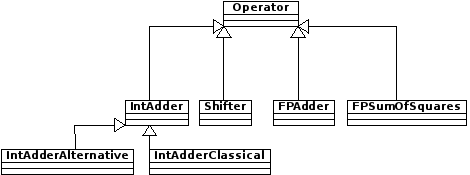
\includegraphics{flopocoClassHierarchy}
 \caption{Extract of the \acs{FloPoCo} class hierarchy}
 \label{fig:flopocoOperators}
\end{figure}




\section{\iflanguage{english}{Compute Systems}{Rechensysteme}}
\label{sec:hardware}

\subsection{AMD Tahiti}

\subsection{Intel Xeon Phi}

\subsection{Nvidia ...}


\section{\iflanguage{english}{Implementation}{Implementierung}}

\subsection{\iflanguage{english}{Designing the Kernel's interface}{Entwurf der 
Schnittstelle des Kernels}}

Many implementations of linear algebra routines in OpenCL strive for maximal 
performance and therefore restrict their operands to special dimensions, sizes 
and layout. If these implementations are integrated into software packages like 
MATLAB, copying and other preprocessing respectively is required to meet the 
implementations' requirements. This in turn hinders performance. Therefore the 
kernel presented here has a more flexible interface eventhough this may provoke 
a slower execution.

In the C++ standard library when abstracting away the actual layout and size of 
a data structure iterators are used. As OpenCL is a C derivative rather than a 
C++ derivative, iterators can not be used directly if they are more complex 
than simple pointers. Instead several parameters are handed over to the kernel 
that define the iterator. In \cite{Volkov2008} the kernel launch overhead has 
been measured for CUDA and in \cite{Dongarra2013} for OpenCL but not with 
respect to the number of parameters passed to the kernel. In 
\cref{fig:kernelLaunchOverhead} the kernel launch overhead for the three major 
hardware platforms mentioned in \cref{sec:hardware} is presented varying the 
number of parameters from one to 32 which should cover the most common kernel 
invocations. The test was done executing an empty kernel several thousand times 
and then averaging the execution time. As one can see there is a linear 
correspondence between the number of kernel arguments and the launch overhead. 
Thus one should use parameters sparingly. To reduce the number of kernel 
arguments 
one could place them in continuous global memory and just pass the address of 
the first. But that requires extra loading from global memory. Therefore it is 
not used here.

\begin{figure}[htbp]
 \centering
 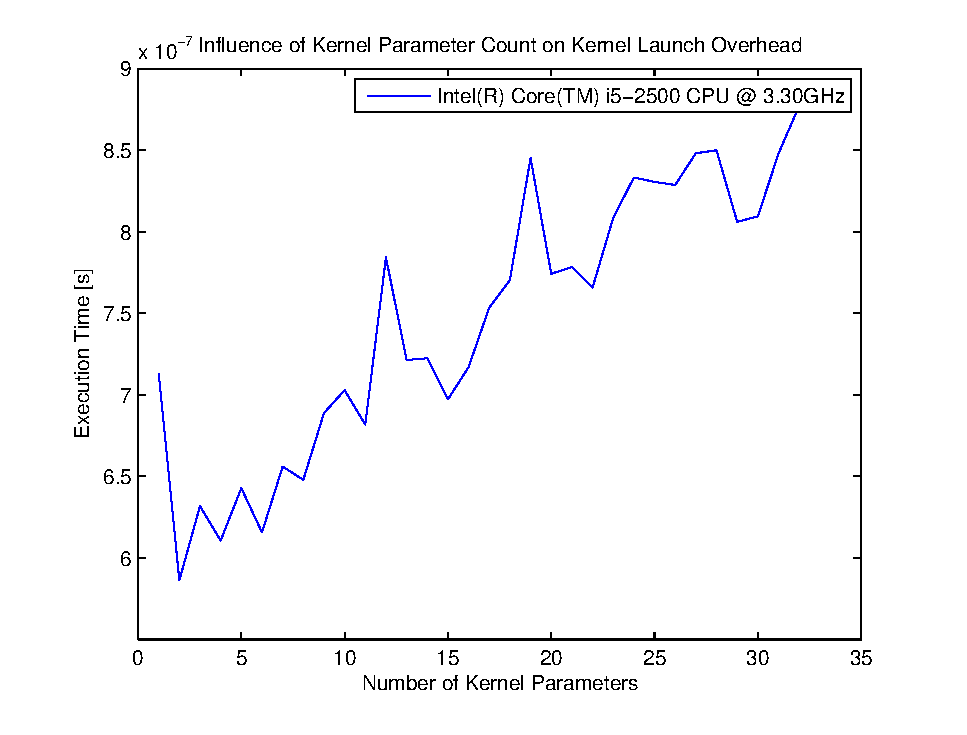
\includegraphics[width=\textwidth]{kernelLaunchOverhead}
 \caption{Impact of the Number of Parameters on Kernel Launch Overhead}
 \label{fig:kernelLaunchOverhead}
\end{figure}

The kernel presented in \cref{lst:kernelHeader} has parameters to access all 
three matrices or submatrices and hides the layout\footnote{This design allows 
column- and row-major layouts only.} of them by additional parameters.

Both operands are qualified with the \texttt{const} keyword to indicate that 
they are read-only. This helps in avoiding unintentional writes and in
optimization. All three pointers are restricted. That enables further 
optimizations on some devices \footnote{E.g.\ AMD Nothern Islands \acp{GPU} 
enable caching only for restricted pointers to read-only 
memory\cite[Section 7.4]{AMD2013}}. The \texttt{restrict} keyword requires that 
\texttt{lhs}, \texttt{rhs} and \texttt{res} do not alias. \texttt{res} must 
point to a distinct memory location because if it was one of the operands 
updating it must be delayed until all reads are done. That would require 
synchronization of all work items which in general is not possible. 
\texttt{lhs} and \texttt{rhs} may alias allowing computations of the form $C = 
A \cdot A$ because they are not updated at all due to the \texttt{const} 
qualifier.

Even though OpenCL does not support templates directly, C++-style 
templatization is used here to indicate that the kernel can be implemented for 
various types.

The offsets mark the beginning of the (sub-) matrices and the stride parameters 
hide column- or row-major data layout of the matrices.

\texttt{innerDim} is the size of the common dimension of the left- and 
right-hand side operand.
\begin{lstlisting}[caption={Interface of the OpenCL kernel for matrix-matrix 
multiplication},label={lst:kernelHeader},language=OpenCL]
template<class T>
kernel void gemm(
  global T const* restrict lhs, // left-hand side (sub-)matrix
  global T const* restrict rhs, // right-hand side (sub-)matrix
  global T* const restrict res, // result (sub-) matrix
  uint const      innerDim,   // inner dimension of lhs and rhs
  uint const      lhsOffset,  // offset into lhs where the 
                              // (sub-) matrix begins
  uint const      rhsOffset,  // same for rhs
  uint const      resOffset,  // same for res
  uint const      lhsStrideX, // distance between consecutive lhs
                              // values in horizontal direction
  uint const      rhsStrideX, // same for rhs
  uint const      resStrideX, // same for res
  uint const      lhsStrideY, // distance between consecutive lhs
                              // values in vertical direction
  uint const      rhsStrideY, // same for rhs
  uint const      resStrideY  // same for lhs
);\end{lstlisting}

Besides global memory OpenCL permits storing data in the texture cache, if the 
device supports that. To make use of the texture cache a second kernel 
interface is presented in \cref{lst:kernelHeaderImgMem}. It supports matrices 
that are stored as textures. On some devices like AMD's Nothern Island 
\acp{GPU} the texture cache has a higher bandwidth than the global memory 
\cite[Section 7.4]{AMD2013}. 

Textures in OpenCL are two- or three-dimensional arrays that store four values 
per texel\footnote{A value for red, green, blue and alpha intensity}. Their 
exact memory layout is not specified such that each implementation can apply 
its own customizations or optimizations respectively. On the other hand images 
stored in host memory are required to be laid out row by row and one to four 
continuous values form one texel. When the image is moved to the texture memory 
missing values are added as specified by the programmer. E.g. if the programmer 
specified that the image in host memory is of the format \texttt{CL\_LUMINANCE} 
then one value in host memory is copied and duplicated into image memory such 
that the resulting texel has the value $\begin{pmatrix}L,L,L,1.0\end{pmatrix}$. 
If the image has been given the channel order \texttt{CL\_RGBA} then four 
values in host memory are copied into one texel in image memory of the form 
$\begin{pmatrix}R,G,B,A\end{pmatrix}$.

As stated above, the layout of images in image memory is not specified. Images 
can not be accessed like arrays inside a kernel but by two- or 
three-dimensional coordinates. Thus the offset parameters slightly differ from 
the kernel in \cref{lst:kernelHeader}. Logically the strides in both direction 
are one. If the matrix was not in row- but in column-major format before 
copying it into image memory this is indicated by the \texttt{transpose} 
parameter.

% TODO Encoding of textures as matrices.

\begin{lstlisting}[caption={Interface of the OpenCL kernel for matrix-matrix 
multiplication using image 
memory},label={lst:kernelHeaderImgMem},language=OpenCL]
kernel void gemm(
  read_only  image2d_t lhs,
  read_only  image2d_t rhs,
  write_only image2d_t res,
  int const            innerDim,
  int const            lhsOffsetX,
  int const            rhsOffsetX,
  int const            resOffsetX,
  int const            lhsOffsetY,
  int const            rhsOffsetY,
  int const            resOffsetY,
  int const            lhsTranspose, // Was the matrix in host
                                     // memory stored in column-
                                     // or row-major format?
  int const            rhsTranspose,
  int const            resTranspose
);\end{lstlisting}


% TODO Test how more parameters influence the time it takes to invoke a kernel.


%----------------------------------------------------------------------
%- Anhang
%----------------------------------------------------------------------

\part{Anhänge}
\appendix

\include{chapter/Appendix}

\section{Abkürzungen}\index{Abkürzungen}
%\section{Abkürzungen}\index{Abkürzungen}
\label{chap:abkuerzungen}
%#############################################
%#############################################
% \begin{table}[ht]
% 		\begin{tabular}{ll}		
% 		\end{tabular}
% \end{table}

\begin{acronym}
\acro{BLAS}{Basic Linear Algebra Subprograms}
\acro{CPU}{Central Processing Unit}
\acro{DLA}{dense linear algebra}
\acro{FloPoCo}{Floating-Point Cores}
\acro{GEMM}{General matrix-matrix multiplication}
\acro{GPU}{Graphics Processing Unit}
\acro{MKL}{Math Kernel Library}
\acro{MPI}{message passing interface}
\acro{Muesli}{Münster Skeleton Library}
\acro{PCI}{Peripheral Component Interconnect}
\acro{PCIe}{\acs{PCI} express}
\acro{SGEMM}{Single-precision \ac{GEMM}}
\acro{STL}{Standard Template Library}
\acro{TLB}{Translation Lookaside Buffer}
\end{acronym}


%#############################################
%#############################################



	% BibTeX Datei mit Literaturliste
	% pdflatex Thesis.tex
	% bibtex Thesis.aux
	% pdflatex Thesis.tex
	% pdflatex Thesis.tex
\sloppy
\bibliographystyle{plain}
\bibliography{bibliography/Literatur}
\nocite{*}

\end{document}

% Ende des Dokuments:----------------------------------------------------------------

